\documentclass[10pt, compress]{beamer}

\usetheme{m}
\usepackage{mathtools}
\usepackage{booktabs}
\usepackage[scale=2]{ccicons}
\usepackage{minted}
\usepackage{graphicx}

\usemintedstyle{trac}

\title{statistical analysis on Flow Splice Graphs}
\subtitle{Labcourse Graph Theory}
\date{\today}
\author{Daniel Mayer, Benjamin Schindler}
\institute{University of Leipzig}
\begin{document}

\maketitle

\begin{frame}[fragile]
  \frametitle{outline}
\begin{itemize}
	\item  Methods
	\begin{itemize}
		\item Software
		\item own Statistics
	\end{itemize}
	\item Results
	\begin{itemize}
		\item task A general statistics
		\item task B categorical statistics on EP True 
	\end{itemize}
	\item Discussion
\end{itemize}
\end{frame}
\begin{frame}[fragile]
	\frametitle{Methods}
	Software:
	\begin{itemize}
		\item scripting in python2
			\begin{itemize}
				\item networkx as graph library
				\item graph data written to CSV
			\end{itemize}
		\item statistics in R using ggplot2
	\end{itemize}
	Source code available at https://github.com/gnummig/labcourse\_graphtheory
\end{frame}
\begin{frame}[fragile]
	\frametitle{own statistics }
	\begin{equation*}
	\leftarrow	
	\end{equation*}
\end{frame}
\begin{frame}[fragile]
	\frametitle{basic statistics}
	Our dataset is EP True:
	\begin{itemize}
		\item no noise	
		\item perfect alignment
	\end{itemize}
	We compare the \textbf{filtered} and the \textbf{splice graph} Graphs
	\begin{itemize}
		\item \~5000 graphs per category
		\item \~125.000 Problem nodes
		\item \~500 Chimaer nodes
	\end{itemize}

\end{frame}
\begin{frame}[fragile]
	\frametitle{basic statistics}
		\begin{figure}
			\includegraphics[width=\linewidth]{basic_capacity.pdf}
			\caption{Capacity for filtered Graph }
		\end{figure}

\end{frame}
\begin{frame}[fragile]
	\frametitle{basic statistics}
		\begin{figure}
			\includegraphics[width=0.49\linewidth]{basic_capacity.pdf}
			\includegraphics[width=0.49\linewidth]{basic_splice_capacity.pdf}
			\caption{Capacity for filtered Graph and Splice Graph}
		\end{figure}

\end{frame}
\begin{frame}[fragile]
	\frametitle{basic statistics}
		\begin{figure}
			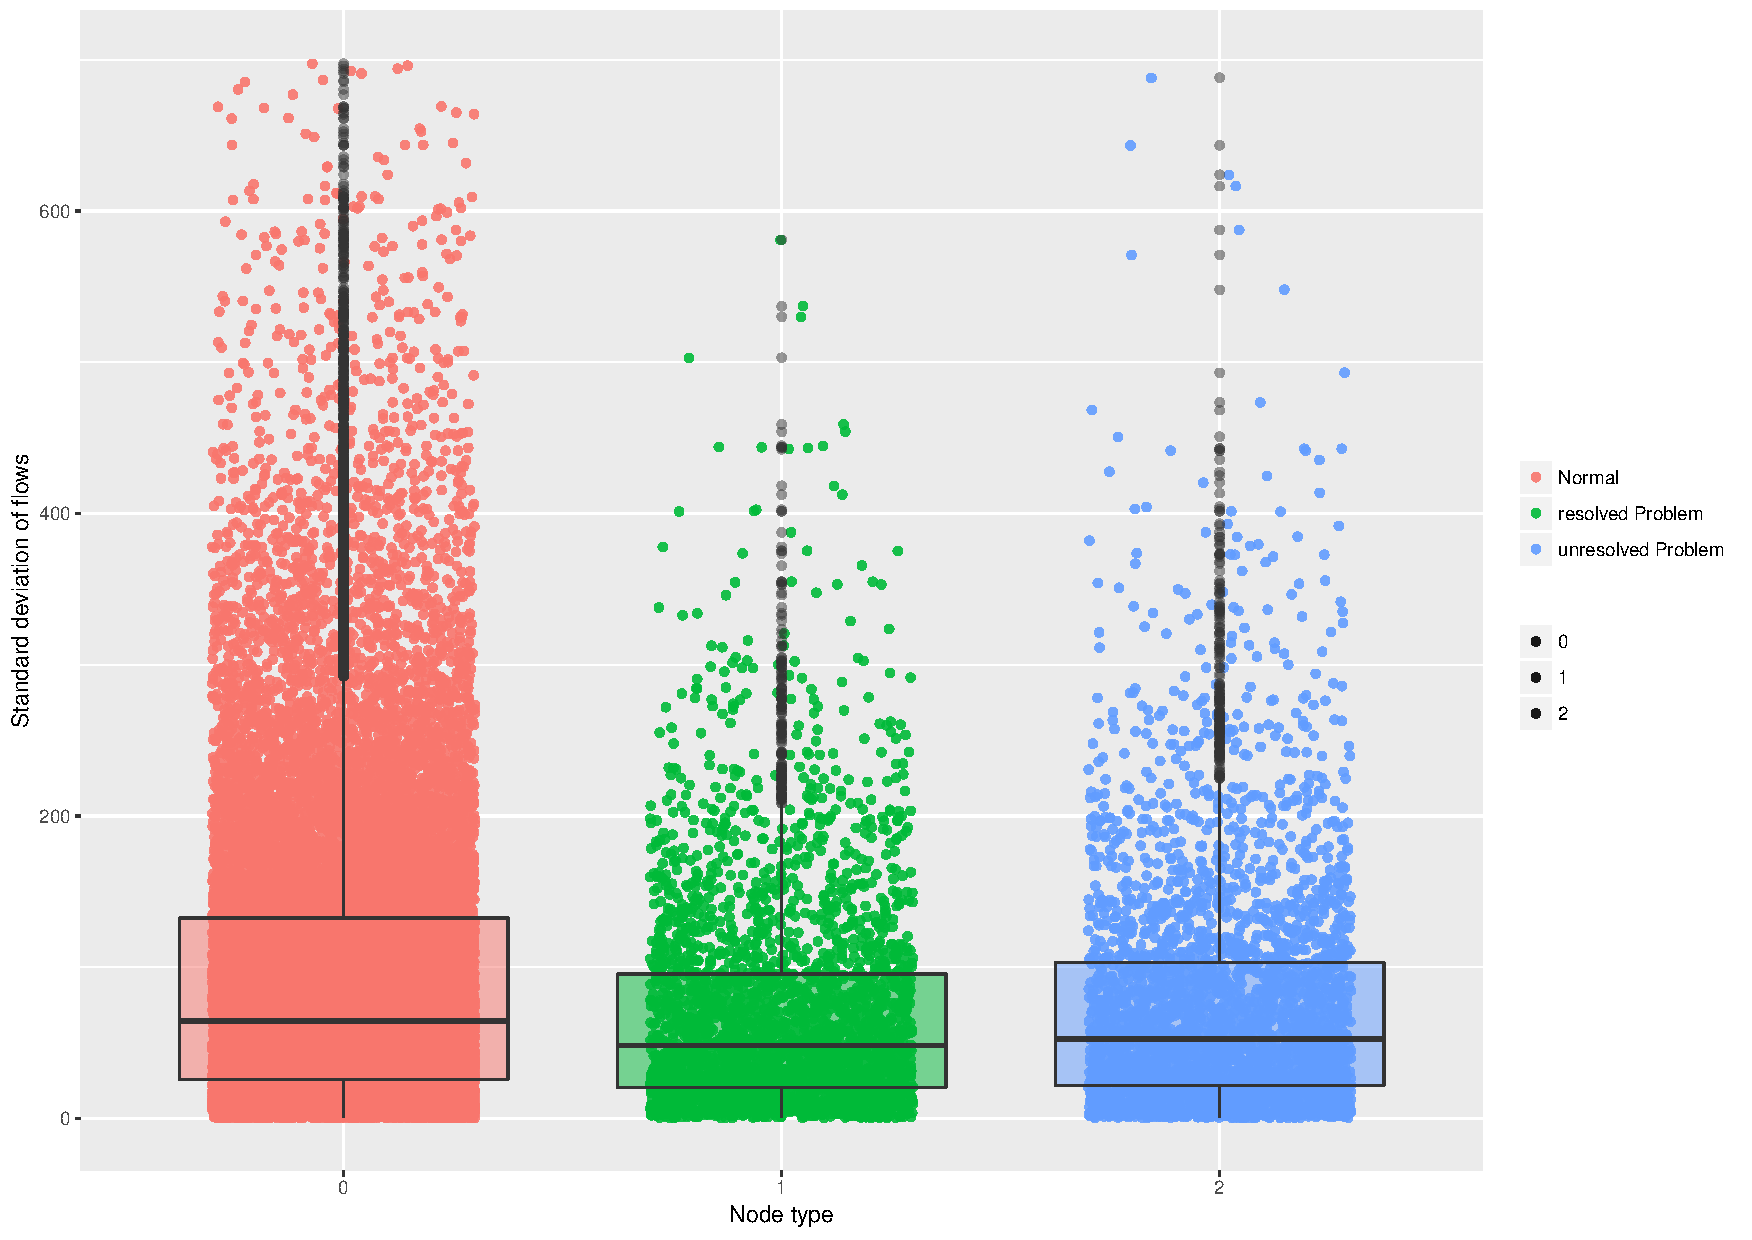
\includegraphics[width=0.49\linewidth]{basic_flowdeviation.pdf}
			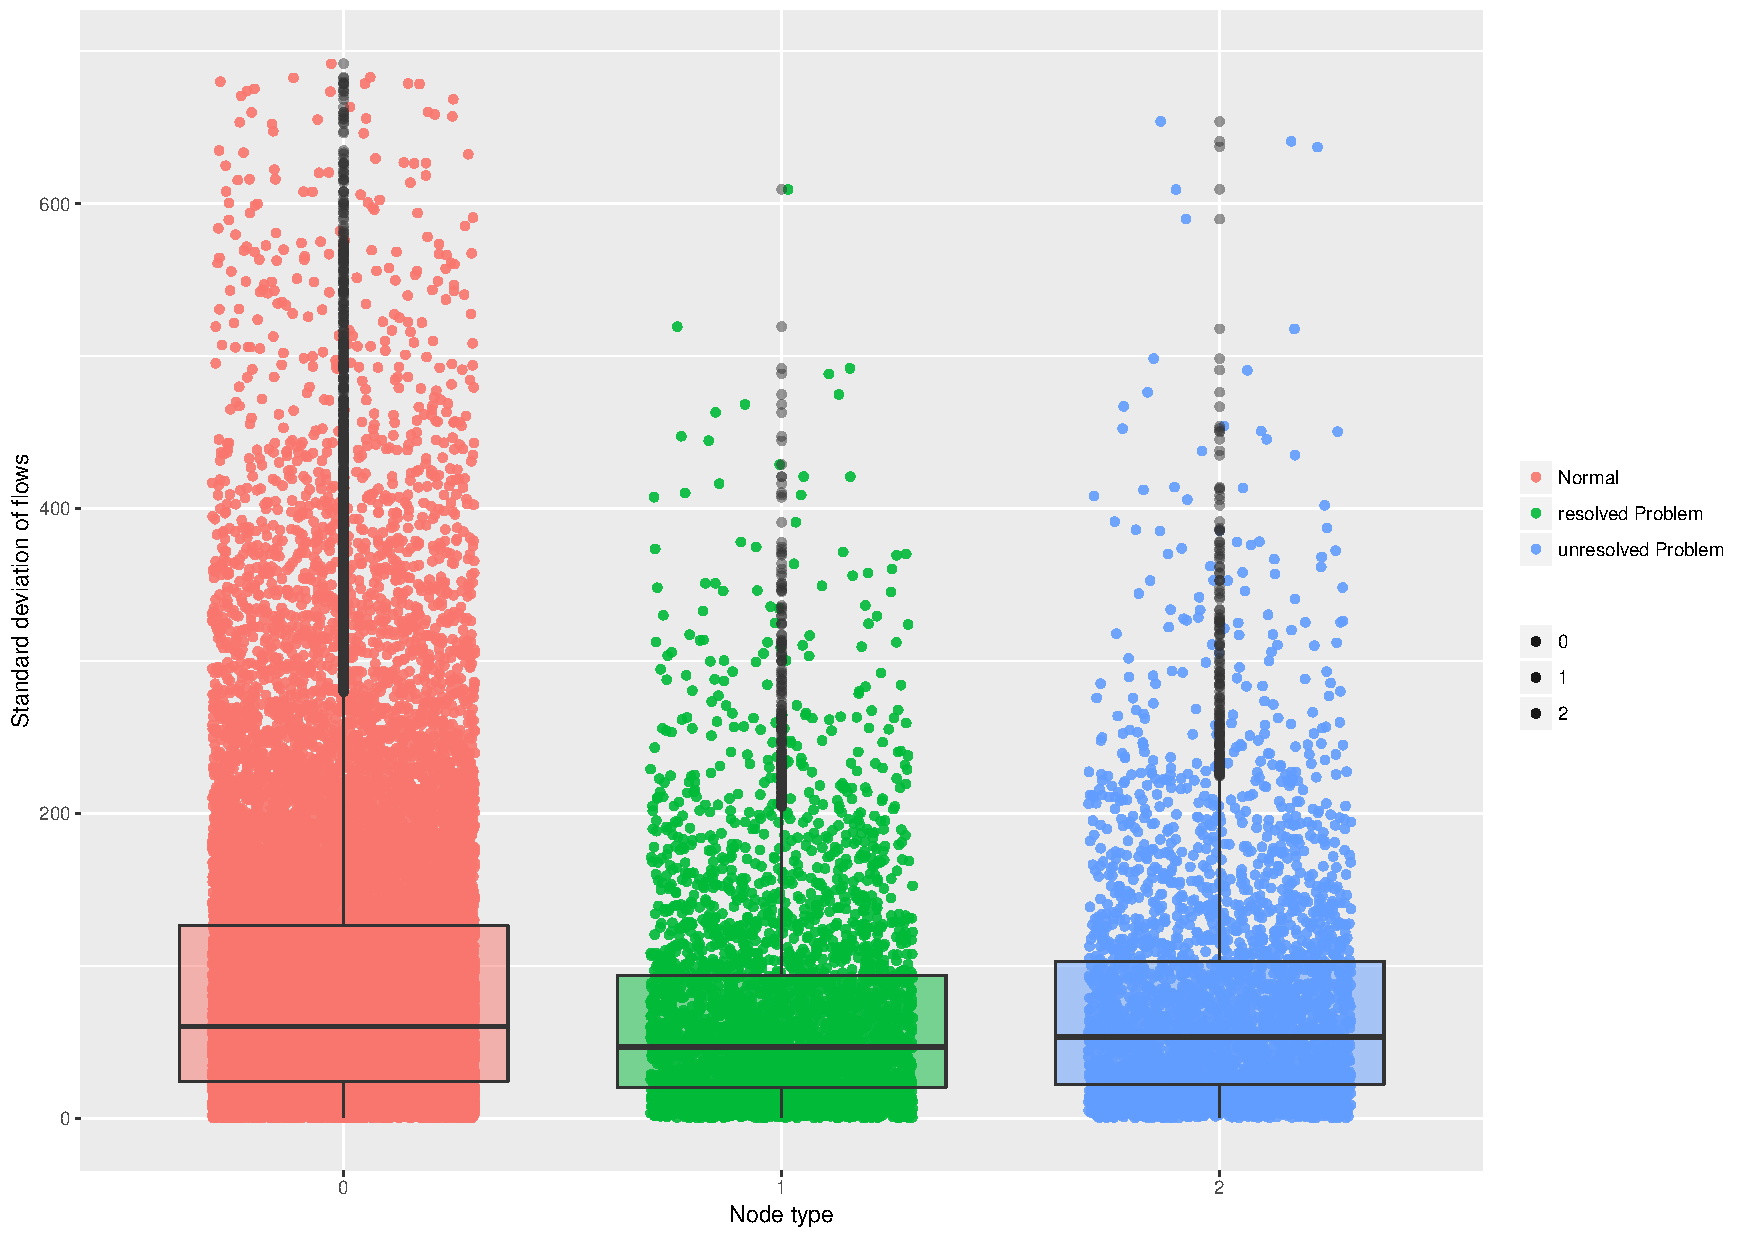
\includegraphics[width=0.49\linewidth]{basic_splice_flowdeviation.pdf}
			\caption{Standard deviation of in and out capacities for filtered Graph and Splice Graph}
		\end{figure}

\end{frame}
\begin{frame}[fragile]
	\frametitle{basic statistics}
		\begin{figure}
			\includegraphics[width=0.49\linewidth]{basic_flowdifference.pdf}
			\includegraphics[width=0.49\linewidth]{basic_splice_flowdifference.pdf}
			\caption{Difference in InCapacity and OutCapacity for filtered Graph and Splice Graph}
		\end{figure}

\end{frame}

\begin{frame}[fragile]
	\frametitle{Chimaer nodes in the context of problem nodes}
	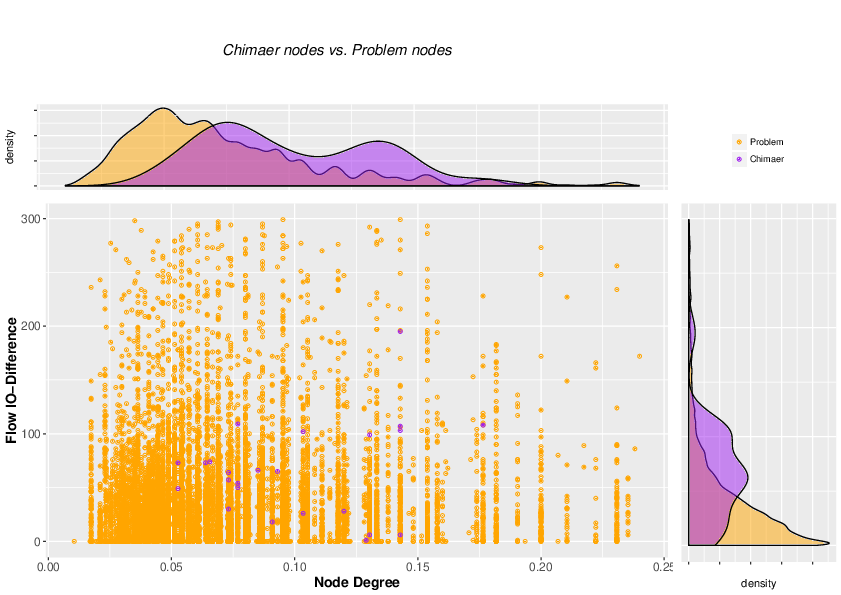
\includegraphics[width=0.9\textwidth]{degree_flowdifference_zoomed_finer.png}
\end{frame}
\begin{frame}[fragile]
	\frametitle{Chimaer nodes in the context of problem nodes}
	\begin{figure}
	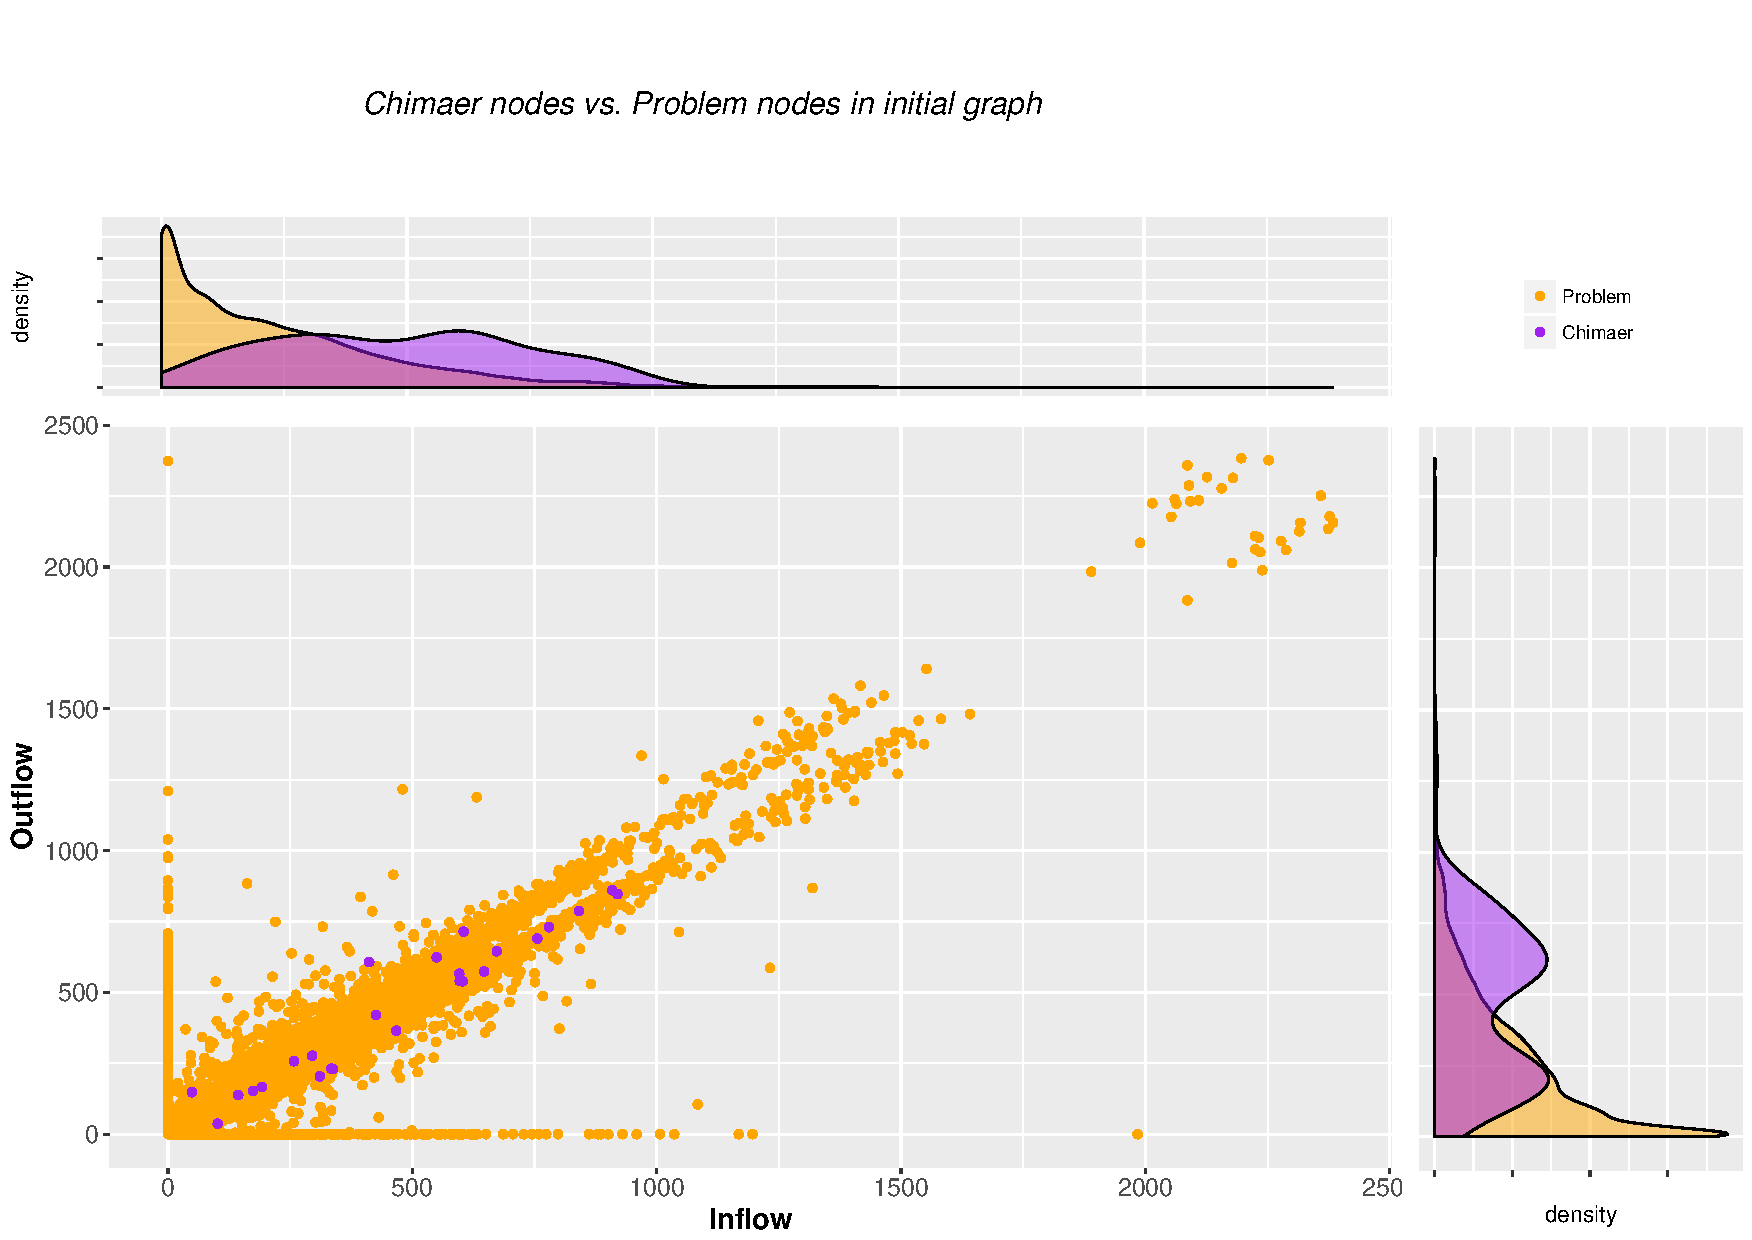
\includegraphics[width=0.9\textwidth]{Inflow_Outflow.pdf}
	\caption{Input flow and output flow for Chimaer and other Problem Nodes}
	\end{figure}
\end{frame}
\begin{frame}[fragile]
        \frametitle{Chimaer nodes in the context of problem nodes}
	\begin{figure}
        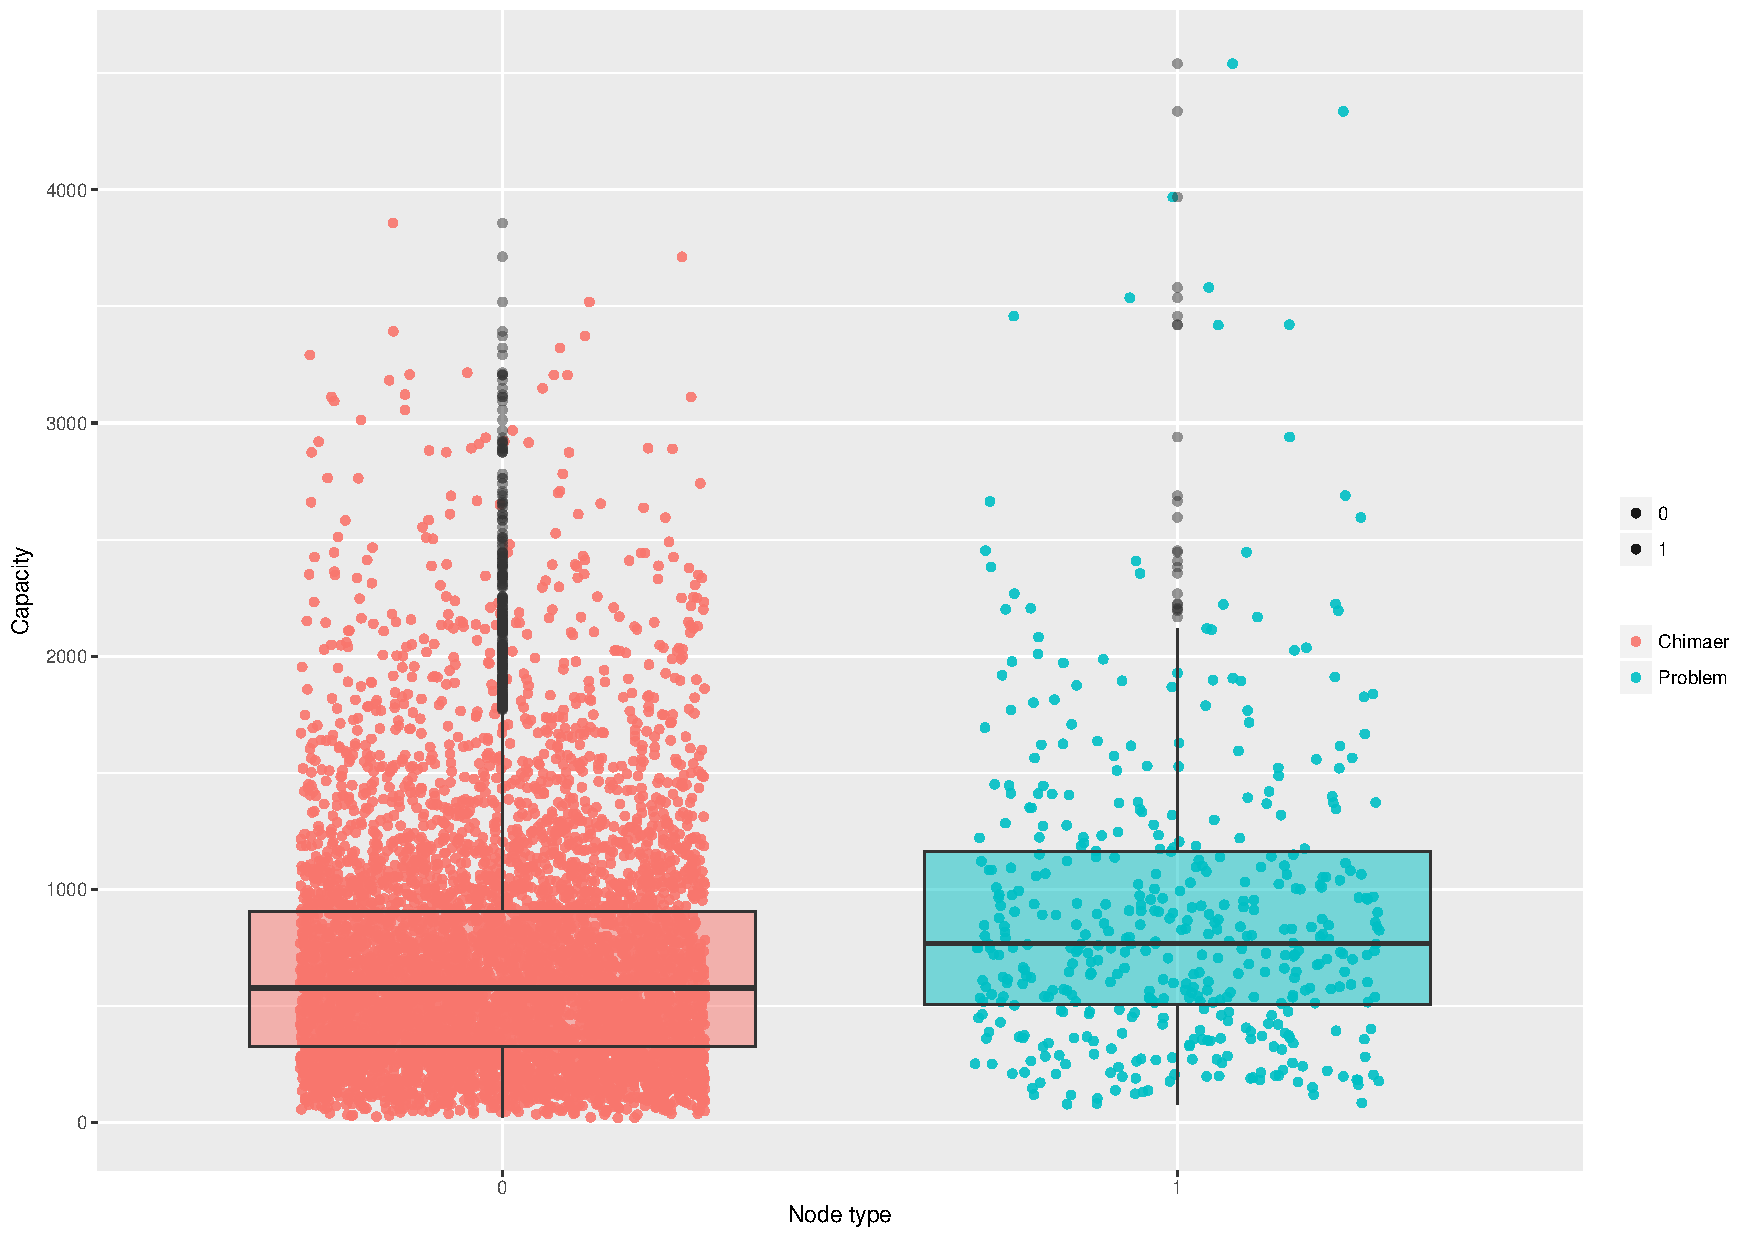
\includegraphics[width=0.9\textwidth]{categorial_flow_filtered.pdf}
	\caption{Capacities for Chimaer and other Problem Nodes}
	\end{figure}
\end{frame}


%\plain{phylogenetic tree of CCA1 and CCA2}{\vspace{-2em}\begin{center}\includegraphics[width=0.9\textwidth]{clodify_tree.png}\end{center}}
%\section{DUF of Laccaria bicolor}
\plain{}{Questions?}
\end{document}
